%  LaTeX support: latex@mdpi.com
%  For support, please attach all files needed for compiling as well as the log file, and specify your operating system, LaTeX version, and LaTeX editor.

%=================================================================
\documentclass[algorithms,article,submit,pdftex,moreauthors]{Definitions/mdpi}
% For posting an early version of this manuscript as a preprint, you may use "preprints" as the journal and change "submit" to "accept". The document class line would be, e.g., \documentclass[preprints,article,accept,moreauthors,pdftex]{mdpi}. This is especially recommended for submission to arXiv, where line numbers should be removed before posting. For preprints.org, the editorial staff will make this change immediately prior to posting.

%--------------------
% Class Options:
%--------------------
%----------
% journal
%----------
% Choose between the following MDPI journals:
% acoustics, actuators, addictions, admsci, adolescents, aerospace, agriculture, agriengineering, agronomy, ai, algorithms, allergies, alloys, analytica, animals, antibiotics, antibodies, antioxidants, applbiosci, appliedchem, appliedmath, applmech, applmicrobiol, applnano, applsci, aquacj, architecture, arts, asc, asi, astronomy, atmosphere, atoms, audiolres, automation, axioms, bacteria, batteries, bdcc, behavsci, beverages, biochem, bioengineering, biologics, biology, biomass, biomechanics, biomed, biomedicines, biomedinformatics, biomimetics, biomolecules, biophysica, biosensors, biotech, birds, bloods, blsf, brainsci, breath, buildings, businesses, cancers, carbon, cardiogenetics, catalysts, cells, ceramics, challenges, chemengineering, chemistry, chemosensors, chemproc, children, chips, cimb, civileng, cleantechnol, climate, clinpract, clockssleep, cmd, coasts, coatings, colloids, colorants, commodities, compounds, computation, computers, condensedmatter, conservation, constrmater, cosmetics, covid, crops, cryptography, crystals, csmf, ctn, curroncol, currophthalmol, cyber, dairy, data, dentistry, dermato, dermatopathology, designs, diabetology, diagnostics, dietetics, digital, disabilities, diseases, diversity, dna, drones, dynamics, earth, ebj, ecologies, econometrics, economies, education, ejihpe, electricity, electrochem, electronicmat, electronics, encyclopedia, endocrines, energies, eng, engproc, ent, entomology, entropy, environments, environsciproc, epidemiologia, epigenomes, est, fermentation, fibers, fintech, fire, fishes, fluids, foods, forecasting, forensicsci, forests, foundations, fractalfract, fuels, futureinternet, futureparasites, futurepharmacol, futurephys, futuretransp, galaxies, games, gases, gastroent, gastrointestdisord, gels, genealogy, genes, geographies, geohazards, geomatics, geosciences, geotechnics, geriatrics, hazardousmatters, healthcare, hearts, hemato, heritage, highthroughput, histories, horticulturae, humanities, humans, hydrobiology, hydrogen, hydrology, hygiene, idr, ijerph, ijfs, ijgi, ijms, ijns, ijtm, ijtpp, immuno, informatics, information, infrastructures, inorganics, insects, instruments, inventions, iot, j, jal, jcdd, jcm, jcp, jcs, jdb, jeta, jfb, jfmk, jimaging, jintelligence, jlpea, jmmp, jmp, jmse, jne, jnt, jof, joitmc, jor, journalmedia, jox, jpm, jrfm, jsan, jtaer, jzbg, kidney, kidneydial, knowledge, land, languages, laws, life, liquids, literature, livers, logics, logistics, lubricants, lymphatics, machines, macromol, magnetism, magnetochemistry, make, marinedrugs, materials, materproc, mathematics, mca, measurements, medicina, medicines, medsci, membranes, merits, metabolites, metals, meteorology, methane, metrology, micro, microarrays, microbiolres, micromachines, microorganisms, microplastics, minerals, mining, modelling, molbank, molecules, mps, msf, mti, muscles, nanoenergyadv, nanomanufacturing, nanomaterials, ncrna, network, neuroglia, neurolint, neurosci, nitrogen, notspecified, nri, nursrep, nutraceuticals, nutrients, obesities, oceans, ohbm, onco, oncopathology, optics, oral, organics, organoids, osteology, oxygen, parasites, parasitologia, particles, pathogens, pathophysiology, pediatrrep, pharmaceuticals, pharmaceutics, pharmacoepidemiology, pharmacy, philosophies, photochem, photonics, phycology, physchem, physics, physiologia, plants, plasma, pollutants, polymers, polysaccharides, poultry, powders, preprints, proceedings, processes, prosthesis, proteomes, psf, psych, psychiatryint, psychoactives, publications, quantumrep, quaternary, qubs, radiation, reactions, recycling, regeneration, religions, remotesensing, reports, reprodmed, resources, rheumato, risks, robotics, ruminants, safety, sci, scipharm, seeds, sensors, separations, sexes, signals, sinusitis, skins, smartcities, sna, societies, socsci, software, soilsystems, solar, solids, sports, standards, stats, stresses, surfaces, surgeries, suschem, sustainability, symmetry, synbio, systems, taxonomy, technologies, telecom, test, textiles, thalassrep, thermo, tomography, tourismhosp, toxics, toxins, transplantology, transportation, traumacare, traumas, tropicalmed, universe, urbansci, uro, vaccines, vehicles, venereology, vetsci, vibration, viruses, vision, waste, water, wem, wevj, wind, women, world, youth, zoonoticdis

%---------
% article
%---------
% The default type of manuscript is "article", but can be replaced by:
% abstract, addendum, article, book, bookreview, briefreport, casereport, comment, commentary, communication, conferenceproceedings, correction, conferencereport, entry, expressionofconcern, extendedabstract, datadescriptor, editorial, essay, erratum, hypothesis, interestingimage, obituary, opinion, projectreport, reply, retraction, review, perspective, protocol, shortnote, studyprotocol, systematicreview, supfile, technicalnote, viewpoint, guidelines, registeredreport, tutorial
% supfile = supplementary materials

%----------
% submit
%----------
% The class option "submit" will be changed to "accept" by the Editorial Office when the paper is accepted. This will only make changes to the frontpage (e.g., the logo of the journal will get visible), the headings, and the copyright information. Also, line numbering will be removed. Journal info and pagination for accepted papers will also be assigned by the Editorial Office.

%------------------
% moreauthors
%------------------
% If there is only one author the class option oneauthor should be used. Otherwise use the class option moreauthors.

%---------
% pdftex
%---------
% The option pdftex is for use with pdfLaTeX. If eps figures are used, remove the option pdftex and use LaTeX and dvi2pdf.
\usepackage{gensymb}
\usepackage{amsmath}
\usepackage{accents}
\usepackage{multirow}
\usepackage{xspace}
\usepackage{subcaption}
\DeclareRobustCommand{\w}{\mbox{\large\ensuremath{\mathsf{w}}}}
\DeclareRobustCommand{\dotp}{\boldsymbol{\cdot}}
\DeclareRobustCommand{\ccirc}{\kern0.5ex\vcenter{\hbox{$\scriptstyle\circ$}}\kern0.5ex}
\DeclareRobustCommand{\e}[1]{{\rm e}^{#1}}
\DeclareRobustCommand{\lay}[1]{^{(#1)}}
\DeclareRobustCommand{\mdot}[1]{\accentset{\mbox{\bfseries .}}{#1}}
\DeclareRobustCommand{\ie}{\emph{i.e.}\@\xspace}
\DeclareRobustCommand{\eal}{et \emph{al.}\@\xspace}
\DeclareRobustCommand{\eg}{e.g.,\@\xspace}
\DeclareRobustCommand{\RMSE}{\text{E}_\text{RMS}}
\DeclareRobustCommand{\AARE}{\text{E}_\text{AAR}}
\DeclareRobustCommand{\R}{\text{R}}
\DeclareRobustCommand{\ps}{\text{s}^{-1}}
\DeclareRobustCommand{\mr}[2]{\multirow{#1}{*}{#2}}
\DeclareRobustCommand{\MPa}{\text{MPa}}

%=================================================================
% MDPI internal commands
\firstpage{1}
\makeatletter
\setcounter{page}{\@firstpage}
\makeatother
\pubvolume{1}
\issuenum{1}
\articlenumber{0}
\pubyear{2022}
\copyrightyear{2022}
%\externaleditor{Academic Editor: Firstname Lastname}
\datereceived{}
%\daterevised{} % Only for the journal Acoustics
\dateaccepted{}
\datepublished{}
%\datecorrected{} % Corrected papers include a "Corrected: XXX" date in the original paper.
%\dateretracted{} % Corrected papers include a "Retracted: XXX" date in the original paper.
\hreflink{https://doi.org/} % If needed use \linebreak
%\doinum{}
%------------------------------------------------------------------
% The following line should be uncommented if the LaTeX file is uploaded to arXiv.org
%\pdfoutput=1

%=================================================================
% Add packages and commands here. The following packages are loaded in our class file: fontenc, inputenc, calc, indentfirst, fancyhdr, graphicx, epstopdf, lastpage, ifthen, lineno, float, amsmath, setspace, enumitem, mathpazo, booktabs, titlesec, etoolbox, tabto, xcolor, soul, multirow, microtype, tikz, totcount, changepage, attrib, upgreek, cleveref, amsthm, hyphenat, natbib, hyperref, footmisc, url, geometry, newfloat, caption

%=================================================================
%% Please use the following mathematics environments: Theorem, Lemma, Corollary, Proposition, Characterization, Property, Problem, Example, ExamplesandDefinitions, Hypothesis, Remark, Definition, Notation, Assumption
%% For proofs, please use the proof environment (the amsthm package is loaded by the MDPI class).

%=================================================================
% Full title of the paper (Capitalized)
\Title{Title}

% MDPI internal command: Title for citation in the left column
\TitleCitation{Title}

% Author Orchid ID: enter ID or remove command
\newcommand{\orcidauthorA}{0000-0001-7367-5453} % Add \orcidA{} behind the author's name
%\newcommand{\orcidauthorB}{0000-0000-0000-000X} % Add \orcidB{} behind the author's name

% Authors, for the paper (add full first names)
\Author{Olivier Pantalé *$^{,\dagger}$\orcidA{}, Firstname Lastname $^{2,\ddagger}$ and Firstname Lastname $^{2,}$*}

%\longauthorlist{yes}

% MDPI internal command: Authors, for metadata in PDF
\AuthorNames{Olivier Pantalé, Firstname Lastname and Firstname Lastname}

% MDPI internal command: Authors, for citation in the left column
\AuthorCitation{Pantalé, O.; Lastname, F.; Lastname, F.}
% If this is a Chicago style journal: Lastname, Firstname, Firstname Lastname, and Firstname Lastname.

% Affiliations / Addresses (Add [XX] after \address if there is only one affiliation.)
\address{%
$^{1}$ \quad Affiliation 1; e-mail@e-mail.com\\
$^{2}$ \quad Affiliation 2; e-mail@e-mail.com}

% Contact information of the corresponding author
\corres{Correspondence: e-mail@e-mail.com; Tel.: (optional; include country code; if there are multiple corresponding authors, add author initials) +xx-xxxx-xxx-xxxx (F.L.)}

% Current address and/or shared authorship
\firstnote{Current address: Affiliation 3.}
\secondnote{These authors contributed equally to this work.}
% The commands \thirdnote{} till \eighthnote{} are available for further notes

%\simplesumm{} % Simple summary

%\conference{} % An extended version of a conference paper

% Abstract (Do not insert blank lines, i.e. \\)
\abstract{}

% Keywords
\keyword{keyword 1; keyword 2; keyword 3 (List three to ten pertinent keywords specific to the article; yet reasonably common within the subject discipline.)}

% The fields PACS, MSC, and JEL may be left empty or commented out if not applicable
%\PACS{J0101}
%\MSC{}
%\JEL{}

%%%%%%%%%%%%%%%%%%%%%%%%%%%%%%%%%%%%%%%%%%
% Only for the journal Diversity
%\LSID{\url{http://}}

%%%%%%%%%%%%%%%%%%%%%%%%%%%%%%%%%%%%%%%%%%
% Only for the journal Applied Sciences
%\featuredapplication{Authors are encouraged to provide a concise description of the specific application or a potential application of the work. This section is not mandatory.}
%%%%%%%%%%%%%%%%%%%%%%%%%%%%%%%%%%%%%%%%%%

%%%%%%%%%%%%%%%%%%%%%%%%%%%%%%%%%%%%%%%%%%
% Only for the journal Data
%\dataset{DOI number or link to the deposited data set if the data set is published separately. If the data set shall be published as a supplement to this paper, this field will be filled by the journal editors. In this case, please submit the data set as a supplement.}
%\datasetlicense{License under which the data set is made available (CC0, CC-BY, CC-BY-SA, CC-BY-NC, etc.)}

%%%%%%%%%%%%%%%%%%%%%%%%%%%%%%%%%%%%%%%%%%
% Only for the journal Toxins
%\keycontribution{The breakthroughs or highlights of the manuscript. Authors can write one or two sentences to describe the most important part of the paper.}

%%%%%%%%%%%%%%%%%%%%%%%%%%%%%%%%%%%%%%%%%%
% Only for the journal Encyclopedia
%\encyclopediadef{For entry manuscripts only: please provide a brief overview of the entry title instead of an abstract.}

%%%%%%%%%%%%%%%%%%%%%%%%%%%%%%%%%%%%%%%%%%
% Only for the journal Advances in Respiratory Medicine
%\addhighlights{yes}
%\renewcommand{\addhighlights}{%

%\noindent This is an obligatory section in “Advances in Respiratory Medicine”, whose goal is to increase the discoverability and readability of the article via search engines and other scholars. Highlights should not be a copy of the abstract, but a simple text allowing the reader to quickly and simplified find out what the article is about and what can be cited from it. Each of these parts should be devoted up to 2~bullet points.\vspace{3pt}\\
%\textbf{What are the main findings?}
% \begin{itemize}[labelsep=2.5mm,topsep=-3pt]
% \item First bullet.
% \item Second bullet.
% \end{itemize}\vspace{3pt}
%\textbf{What is the implication of the main finding?}
% \begin{itemize}[labelsep=2.5mm,topsep=-3pt]
% \item First bullet.
% \item Second bullet.
% \end{itemize}
%}

%%%%%%%%%%%%%%%%%%%%%%%%%%%%%%%%%%%%%%%%%%
\begin{document}

%%%%%%%%%%%%%%%%%%%%%%%%%%%%%%%%%%%%%%%%%%%
%\setcounter{section}{-1} %% Remove this when starting to work on the template.
%\section{How to Use this Template}
%
%The template details the sections that can be used in a manuscript. Note that the order and names of article sections may differ from the requirements of the journal (e.g., the positioning of the Materials and Methods section). Please check the instructions on the authors' page of the journal to verify the correct order and names. For any questions, please contact the editorial office of the journal or support@mdpi.com. For LaTeX-related questions please contact latex@mdpi.com.%\endnote{This is an endnote.} % To use endnotes, please un-comment \printendnotes below (before References). Only journal Laws uses \footnote.
%
%% The order of the section titles is different for some journals. Please refer to the "Instructions for Authors” on the journal homepage.
%

%------------------------------------------------------------------------------------
\section{Introduction}\label{sec:Introduction}
%------------------------------------------------------------------------------------

Numerical methods for simulating the behavior of structures subjected to high thermomechanical loads, as in the case of high-temperature forming of metallic materials, are generally based on the use of commercial Finite Element (FE) codes such as Abaqus or laboratory codes such as DynELA \cite{Pantale-2004-DOF}, which has been developed at LGP for many years.
These simulation softwares are based on two types of equations: conservation equations and constitutive equations.
If the first equations are generally well established on the basis of physics and mechanics, it is not the same for the second type of equations: the constitutive equations.
Thus, in a general way, the conservation equations concern the fundamental principles of physics such as the mass conservation law, the momentum law (fundamental equation) and the energy law (declined in the form of the first and second principles of thermodynamics).
By themselves, these laws are not sufficient to describe the behavior of a material or a structure subjected to thermomechanical stresses, because the nature of the material's behavior, generally translated by means of the behavior laws, is not included in the system previously proposed.
Therefore, for each type of material, it is necessary to define behavior laws whose formulation is based on observation, in order to describe the behavior of this material under external stresses.
The quality and the accuracy of the results of any numerical simulation depend on the choice of these behavior laws and on the ability of the user to identify the coefficients of these behavior laws for a given material by performing experiments under conditions close to those encountered during the real stress of the structure in service that one wishes to design.
Depending on the nature of the stresses, these tests are based on quasi-static or dynamic tensile or compression tests, tests on thermomechanical simulators such as Gleeble or impact tests using gas launchers or Hopkinson bars.

Generally speaking, in the context of thermomechanical simulation of forming processes, these behavior laws define the dependence of the flow stress of the material $\sigma^y$ as a function of the three input variables which are the plastic strain $\varepsilon^p$, the strain rate $\mdot\varepsilon$ and the temperature $T$ of the material.
These laws, due to the nature of materials and the phenomena involved (work hardening, movement of dislocations, structural hardening, phase transformations, ...) are highly non-linear and their validity is restricted to a certain range of strains, strain rates and temperatures.
From the observations made, we can define two main classes of behavior laws: the flow laws based on physics and the empirical flow laws.
From the mechanics of continuous media and experimental tests and depending on the nature of the materials used, a number of flow models have been developed in the past, including: the Johnson-Cook flow law \cite{Johnson-1983}, the Zerilli Armstrong flow law \cite{Zerilli-1987} and their respective derived forms \cite{Rule-1998, Lin-2010, Li-2013, Zhang-2015, Zhou-2019}, the Hansel-Spittle \cite{Hensel-1978} or the Arrhenius \cite{Jonas-1969} flow laws, to name only a few of the most widely used in the context of the shaping of metallic materials at high temperature.
Once the choice has been made concerning the type of flow law to be used for a given material, it is then necessary, from a set of experimental tests carried out in the laboratory under conditions close to those of the structure in service, to identify the parameters of these flow laws by machine learning methods based on approaches of minimization of the calculated experiment.

The main problem that the researchers are confronted with after the phase of realization of the experimental tests concerns the choice of the flow law to use according to the observations made on these test results.
This choice of flow law is also restricted by the nature of the FE code used.
Thus, a user of the Abaqus FE code, will turn more particularly to a flow law of the Johnson-Cook \cite{Johnson-1983} type insofar as it is natively implemented in this software.
The choice of another form of flow law (Zerilli-Armstrong, or Arrhenius for example) obliges the user to program himself the computation of the flow stress $\sigma^y$ of the material by means of a VUMAT routine in FORTRAN as proposed by Liang \eal \cite{Liang-2022} for an Arrhenius type flow law.
The implementation of this VUMAT subroutine also requires the computation of the derivatives of the flow stress $\sigma^y$ with respect to the three input variables $\varepsilon^p$, $\mdot\varepsilon$ and $T$ which can quickly become relatively complex as the complexity of the flow law increases.
The choice of this flow law is therefore doubly guided by the nature of the behavior of the material on the one hand, but especially by the list of flow laws implemented natively in the FE codes.
At this time, there is not yet a flow law generic enough to cover a wide range of material behavior.

Depending on the nature of the study, the choice of this flow law is generally guided mainly by the list of flow laws available in the Finite Element code used, and very often this choice is made at the expense of the quality of the model.
For example, Zhou \eal \cite{Zhou-2019}, proposed the identification of the flow law of a GCr15 alloy for a continuous casting bloom with heavy reduction application.
In their study, they performed compression tests on GCr15 cylinders in a temperature range of $750~\celsius$ to $1300~\celsius$, strain rates of $0.001~\ps$ to $0.1~\ps$ and strains of $0$ to $0.7$.
The results of these compression tests, plotted in Figure \ref{fig:Zhou-OriginalData}, show a decrease in flow stress $\sigma^y$ with respect to temperature $T$ and a growth of $\sigma^y$ with respect to strain rate $\mdot\varepsilon$, as in most metallic materials.
\begin{figure}[!ht]
\centering
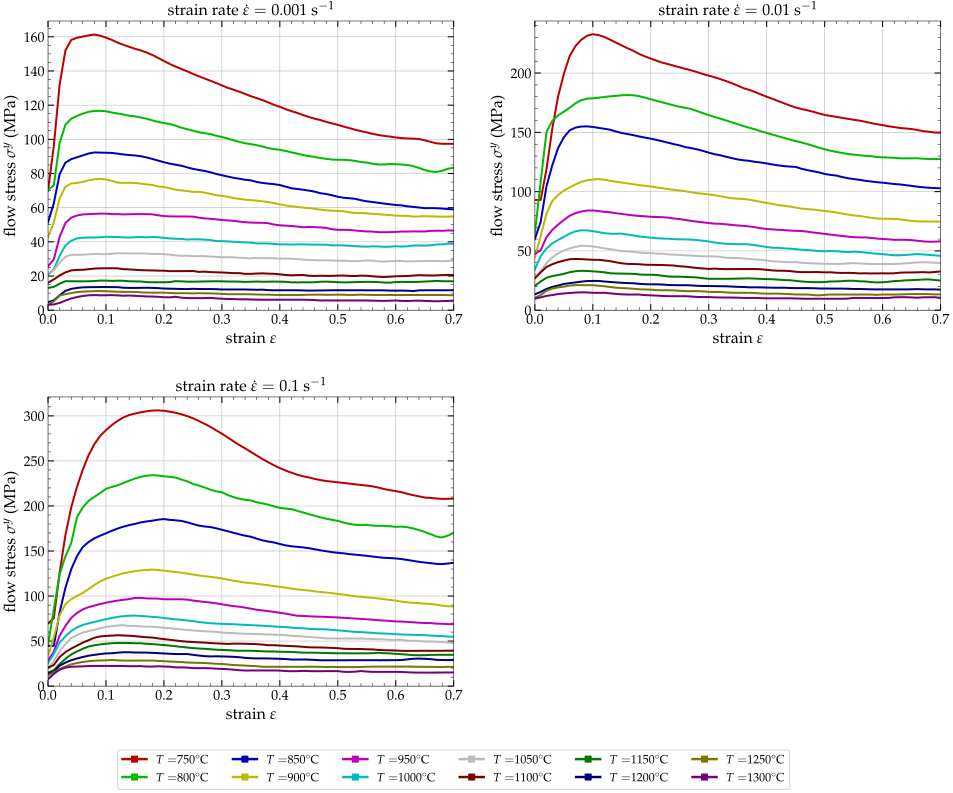
\includegraphics[width=0.9\columnwidth]{Figures/Zhou-OriginalData}
\caption{Original Data.}
\label{fig:Zhou-OriginalData}
\end{figure}
The evolution of the flow stress as a function of the plastic deformation shows the presence of a dynamic recrystallization phenomenon (DRX) within the material.
This phenomenon is an additional non-linearity of this type of material compared to other materials, mainly due to high temperatures and low strain rates, which should be taken into account when describing the material behavior.
As stated in their publication, depending on the flow model used: Johnson-Cook, Modified Zerilli-Armstrong, Arrhenius or new Modified Johnson-Cook, the fidelity of taking into account the real behavior varies widely with the complexity of the flow model which includes between $5$ parameters for the Johnson-Cook model, and up to $16$ parameters for the Arrhenius model.
Thus, and for the input data used, the two most common models: Johnson-Cook and Zerilli-Armstrong do not correctly describe the material behavior.
Only the modified Johnson-Cook and Arrhenius models are able to describe the behavior correctly.
Unfortunately, and this is not part of their study, if these last two models are satisfactory from a theoretical point of view, from a practical point of view for the user of a FE code such as Abaqus, it will be necessary to carry out a numerical implementation in a FORTRAN VUMAT subroutine of the modified Johnson-Cook flow law or the Arrhenius law as carried out by Liang \eal \cite{Liang-2022} in order to be able to use these laws for numerical simulation.
This requires a certain expertise in the development and implementation of flow laws, which is not available to all users of the Abaqus FE code.

From this observation, and from the necessity to select a flow law for a given type of material, then to identify the parameters of this flow law according to experimental tests, and finally to implement this flow law in the form of a user subroutine in FORTRAN in the Abaqus FE code, we have recently proposed in Pantalé \eal \cite{Pantale-2021} an alternative approach based on the ability of Artificial Neural Networks (ANNs) to behave as universal approximators.
The underlying idea is to implement a flow law described by an ANN in the form of a FORTRAN subroutine in the Abaqus FE code.
This neural network was previously trained from the data extracted from mechanical tests of the material and can directly define the value of the flow stress $\sigma^y$ as a function of the plastic strain $\varepsilon^p$, the strain rate $\mdot\varepsilon$ and the temperature $T$.
After this learning phase based on the use of the Python library Tensorflow \cite{Abadi-2016}, the weights and biases of the neural network are transcoded into a subroutine in FORTRAN which is compiled and linked with the libraries of the Abaqus FE code in order to include the behavior of the material by allowing the computation of the flow stress $\sigma^y$ as a function of $\varepsilon^p$, $\mdot\varepsilon$ and $T$, and of its three derivatives $\partial\sigma^y/\partial\varepsilon^p$, $\partial\sigma^y/\partial\mdot\varepsilon$ and $\partial\sigma^y/\partial T$.

The structure of this paper is as follows.
Section \ref{sec:Training} deals with the presentation of a Neural Network based flow law and its training from the data reported in figure \ref{fig:Zhou-OriginalData}.
The comparison of several neural network architectures regarding accuracy and implementation complexity will be presented.
In Section \ref{sec:Implementation}, we will present the conversion of this neural network into FORTRAN and C++ subroutines for Abaqus and DynELA FE codes.
Section \ref{sec:Simulations} will present real test cases of the use of an ANN flow law in numerical simulations and the comparison between the implementations made on Abaqus and DynELA.
Finally, a conclusion and perspective section will be presented at the end.


%------------------------------------------------------------------------------------
\section{Training of the ANN flow law}\label{sec:Training}
%------------------------------------------------------------------------------------

In this section, we briefly recall, as an introduction, some basic principles of Artificial Neural Networks that are relevant to this work.
The global architecture chosen to model the behavior of a material is based on a multi-layer feed-forward ANN which as proposed by Hornik \eal \cite{Hornik-1989-MFN} can be used as a universal approximator.
The architecture retained for this study concerns a neural network with two hidden layers containing a variable number of neurons on these two layers, $3$ inputs corresponding to the plastic strain $\varepsilon^p$, the strain rate $\mdot\varepsilon$ and the temperature $T$ respectively and a single output concerning the flow stress of the material $\sigma^y$.
Figure \ref{fig:ANN-scheme} shows a graphical representation of the global architecture of this neural network.
\begin{figure}[!ht]
\centering
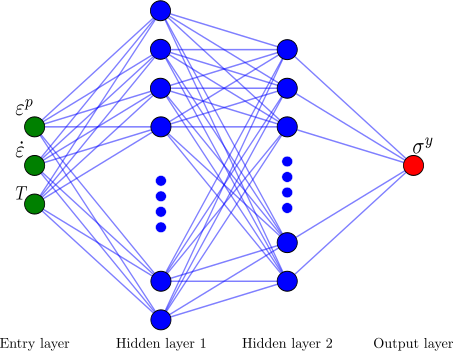
\includegraphics[width=0.7\columnwidth]{Figures/ANN-scheme-2HL}
\caption{Global structure of the ANN flow law with two hidden layers, 3 inputs and one output.}
\label{fig:ANN-scheme}
\end{figure}
The choice of the number of neurons in the two hidden layers is free, but must be reasonable.
Indeed, the more neurons the network contains, the more it will be able to reproduce faithfully the training data, but the less it will be able to generalize to new data (the classical problem of overlearning of neural networks).
Moreover, the more neurons it contains, the more complex its mathematical structure will be, and the more computation time it will require within the routine included in the FE code.
It is therefore necessary to respect a balance between the capacity of the network to minimize errors during the learning phase, its complexity and the speed of execution once it is transcribed into the FE code.

%------------------------------------------------------------------------------------
\subsection{Neural Network governing equations}\label{sec:ANN-equations}
%------------------------------------------------------------------------------------

According to Figure \ref{fig:ANN-scheme}, the neural network has $3$ inputs (referred as the input vector $\overrightarrow{x}$ of the ANN) corresponding to the plastic strain $\varepsilon^p$, the strain rate $\mdot\varepsilon$ and the temperature $T$ respectively.
These inputs are first normalized within the range $[0,1]$ in order to avoid a ill-conditioning of the system as presented by many other authors in the literature \cite{Lin-2008-ANN, Lu-2011-ANN} since these three variables represent different physical data with a very different amplitudes ($0.7$ for the plastic strain, $100$ for the strain rate and $550~\celsius$ for the temperature in the case of the data reported in Figure \ref{fig:Zhou-OriginalData}).
Therefore, the three components of the input vector $\overrightarrow{x}$ are obtained from the plastic strain $\varepsilon^p$, the strain rate $\mdot\varepsilon$ and the temperature $T$ using the following expressions:
\begin{equation}
\overrightarrow{x}=
\begin{cases}
x_1 = \frac{\varepsilon^p - [\varepsilon^p]_{min}}{[\varepsilon^p]_{max} - [\varepsilon^p]_{min}}\\
x_2 = \frac{\ln(\mdot\varepsilon/\mdot\varepsilon_0)-[\ln(\mdot\varepsilon/\mdot\varepsilon_0)]_{min}}{[\ln(\mdot\varepsilon/\mdot\varepsilon_0)]_{max}-[\ln(\mdot\varepsilon/\mdot\varepsilon_0)]_{min}}\label{eq:CR1}\\
x_3 = \frac{T-[T]_{min}}{[T]_{max}-[T]_{min}}
\end{cases}
\end{equation}
where $[~]_{min}$ and $[~]_{max}$  are the boundaries of the range of the corresponding field.
Concerning the strain rate $\mdot\varepsilon$, and taking into account that its amplitude in a real case can reach $10^5~\ps$, as proposed in Pantalé \cite{Pantale-2021}, we chose at first to substitute $\ln(\mdot\varepsilon/\mdot\varepsilon_0)$, with $\mdot\varepsilon_0$ equal to the lowest strain rate test, for the value of $\mdot\varepsilon$.
After normalization, these three input variables are introduced into the neural network and are propagated within it by the feed-forward propagation mechanism.

Conforming to the structure of the ANN reported in Figure \ref{fig:ANN-scheme} any hidden layer $k$, containing $n$ neurons, takes a weighted sum of the outputs $\overrightarrow{\hat{y}}$ of the immediately previous layer $(k-1)$, containing $m$ neurons, given by the following equation:
\begin{equation}
y_i\lay{k} = \sum_{j=1}^m w_{ij}\lay{k} \hat{y}_j^{(k-1)}+ b_i\lay{k},\label{eq:ANN1}
\end{equation}
where $y_i\lay{k}$ is the entry of the $i^{th}$ neuron of layer $k$, $\hat{y}_j\lay{k-1}$ is the output of the $j^{th}$ neuron of layer $(k-1)$, $w_{ij}\lay{k}$ is the associated weight parameter between the $i^{th}$ neuron of layer $k$ and the $j^{th}$ neuron of layer $(k-1)$ and $b_i\lay{k}$ is the associated bias of the $i^{th}$ neuron of layer $k$.
Those weights $w_{ij}$ and bias $b_i$, for each layer, are the training parameters of the ANN that we have to adjust during the training process.
For the proposed model, we have selected the Sigmoid activation function, so that, each neuron in the hidden layer $k$ provides an output value ${\hat{y}}$ from the input value $y$ of the same neuron defined by Equation (\ref{eq:ANN1}) according to the following equation:
\begin{equation}
\hat{y}=\frac{1}{1 + \e{-y}}\label{eq:ANN2}
\end{equation}

According to equations (\ref{eq:ANN1}) and (\ref{eq:ANN2}), the output of each of the two hidden layers is given by the following two equations:
\begin{equation}
\overrightarrow{y}_1 = \left[1 + \exp{\left(- \w_1 \dotp \overrightarrow{x}- \overrightarrow{b}_1\right)}\right]^{-1}\label{eq:ANN3}
\end{equation}
\begin{equation}
\overrightarrow{y}_2 = \left[1 + \exp{\left(- \w_2 \dotp \overrightarrow{y}_1- \overrightarrow{b}_2\right)}\right]^{-1}\label{eq:ANN4}
\end{equation}
Then we compute the output $s$ of the ANN from the output vector of the second hidden layer $\overrightarrow{y}_2$ using the following equation:
\begin{equation}
s = \overrightarrow{w}^T \dotp \overrightarrow{y}_2 + b\label{eq:ANN5}
\end{equation}
Finally, since no activation function is used for the output neuron of the ANN as usually done in regression ANN, the flow stress $\sigma^y$ can be obtained from the output $s$ using the following equation:
\begin{equation}
\sigma^y =  \left([\sigma]_{max}-[\sigma]_{min}\right)s + [\sigma]_{min} \label{eq:CR2}
\end{equation}

%------------------------------------------------------------------------------------
\subsection{Computation of the derivatives of the Neural Network}\label{sec:ANN-derivative}
%------------------------------------------------------------------------------------

As introduced in Section \ref{sec:Introduction}, the implementation of a flow law in a FE code requires both the computation of the flow stress $\sigma^y$ as a function of the input data, but also the evaluation of the three derivatives of $\sigma^y$ with respect to the input data in order to be able to use a Newton-Raphson algorithm within the stress integration scheme, as proposed by Ming \eal \cite{Ming-2018-ERV, Liang-2022} based on the radial return algorithm in the Abaqus or DynELA FE codes.
It is therefore necessary to perform a numerical evaluation of these three derivatives based on the ANN in order to obtain these quantities.
It seems obvious that it is not possible to train a neural network to evaluate these values of derivatives insofar as the training data are not physically collectible data during the experimental tests.
It is therefore necessary to predict these derivatives from the neural network architecture itself.
One straightforward, but not recommended, solution to this problem is to numerically compute the derivative of $\sigma^y$ with respect to $\varepsilon^p$, $\mdot\varepsilon$ and $T$ using the following relation:
\begin{equation}
\frac{\partial \sigma(x)}{\partial x} = \frac{\sigma(x+\delta x) - \sigma(x)}{\delta x}
\end{equation}
where $\delta x$ is a small increase ($\delta x=10^{-6}$ for example) applied to one of the $3$ variables $\varepsilon^p$, $\mdot\varepsilon$ and $T$.
We need to compute $4$ times a result from the ANN to compute the flow stress and approximate the three derivatives which is quite time-consuming.
The solution for this study consists, insofar as the architecture of the neural network is known through equations \ref{eq:ANN1} to \ref{eq:ANN5}, in analytically deriving the output $s$ of the network with respect to the input $\overrightarrow{x}$, then integrating the data normalization operations defined by equations \ref{eq:CR1} and \ref{eq:CR2}.
Given equations \ref{eq:CR1} to \ref{eq:CR2}, we can then establish in the case of a neural network containing two hidden layers and a sigmoid activation function on the two hidden layers that the derivative of $\sigma^y$ with respect to the input data $\varepsilon^p$, $\mdot\varepsilon$ and $T$ is given by the following equations. First we compute the internal terms of the ANN to compute the derivative of the ANN with respect to the input vector $\overrightarrow{x}$:
\begin{equation}
\begin{cases}
\overrightarrow{z}_1 = \exp{\left(- \w_1 \dotp \overrightarrow{x}- \overrightarrow{b}_1\right)}\\
\overrightarrow{z}_2 = \exp{\left(\w_2 \dotp \frac{1}{1+\overrightarrow{z}_1} + \overrightarrow{b}_2\right)}\\
\overrightarrow{z}_3 = \overrightarrow{w} \ccirc \frac{ \overrightarrow{z}_2}{\left(1 + \overrightarrow{z}_2\right)^2}\\
\overrightarrow{z}_4 = \frac{\overrightarrow{z}_1}{\left(1+\overrightarrow{z}_1\right)^2}
\end{cases}
\label{eq:DANN1}
\end{equation}
Then, from the two terms $\overrightarrow{z}_3$ and $\overrightarrow{z}_4$ we can therefore compute the three derivatives of the output $s$ with respect to the input vector $\overrightarrow{x}$ with the following equation where $\overrightarrow{s}'$ is a vector of $3$ components containing the $3$ derivatives $\partial s/\partial\varepsilon^p$, $\partial s/\partial\mdot\varepsilon$ and $\partial s/\partial T$:
\begin{equation}
\overrightarrow{s}' = \w_1^T \dotp \left[\left(\w_2^T \dotp \overrightarrow{z}_3 \right) \ccirc \overrightarrow{z}_4\right]\label{eq:DANN2}
\end{equation}
Finally, from Equation (\ref{eq:DANN2}) and conforming to the normalization of the inputs introduced earlier, one can obtain the $3$ derivatives of the yield stress $\sigma^y$ with respect to the three inputs $\varepsilon^p$, $\mdot\varepsilon$ and $T$ using the following final equation:
\begin{equation}
\begin{cases}
\partial \sigma/\partial \varepsilon^p = s'_1 \frac{[\sigma]_{max} -[\sigma]_{min}}{[\varepsilon^p]_{max} -[\varepsilon^p]_{min}}\\
\partial \sigma/\partial\mdot\varepsilon = \frac{s'_2}{\mdot\varepsilon} \frac{[\sigma]_{max} -[\sigma]_{min}}{[\mdot\varepsilon]_{max} -[\mdot\varepsilon]_{min}} \\
\partial \sigma/\partial T = s'_3 \frac{[\sigma]_{max} -[\sigma]_{min}}{[T]_{max} -[T]_{min}}
\end{cases}
\label{eq:DANN3}
\end{equation}

Equations (\ref{eq:DANN1}-\ref{eq:DANN3}) defines the derivatives of the yield stress $\sigma^y$ with respect to $\varepsilon^p$, $\mdot\varepsilon$ and $T$, as computed by the ANN, and, as shown in \cite{Pantale-2021}, these derivatives can be used for the numerical implementation of the ANN constitutive law in a FE code.

%------------------------------------------------------------------------------------
\subsection{Training of the Neural Network}\label{sec:ANN-traning}
%------------------------------------------------------------------------------------

%------------------------------------------------------------------------------------
\section{Implementation of the ANN flow law in FE softwares}\label{sec:Implementation}
%------------------------------------------------------------------------------------

\begin{figure}[!ht]
\centering
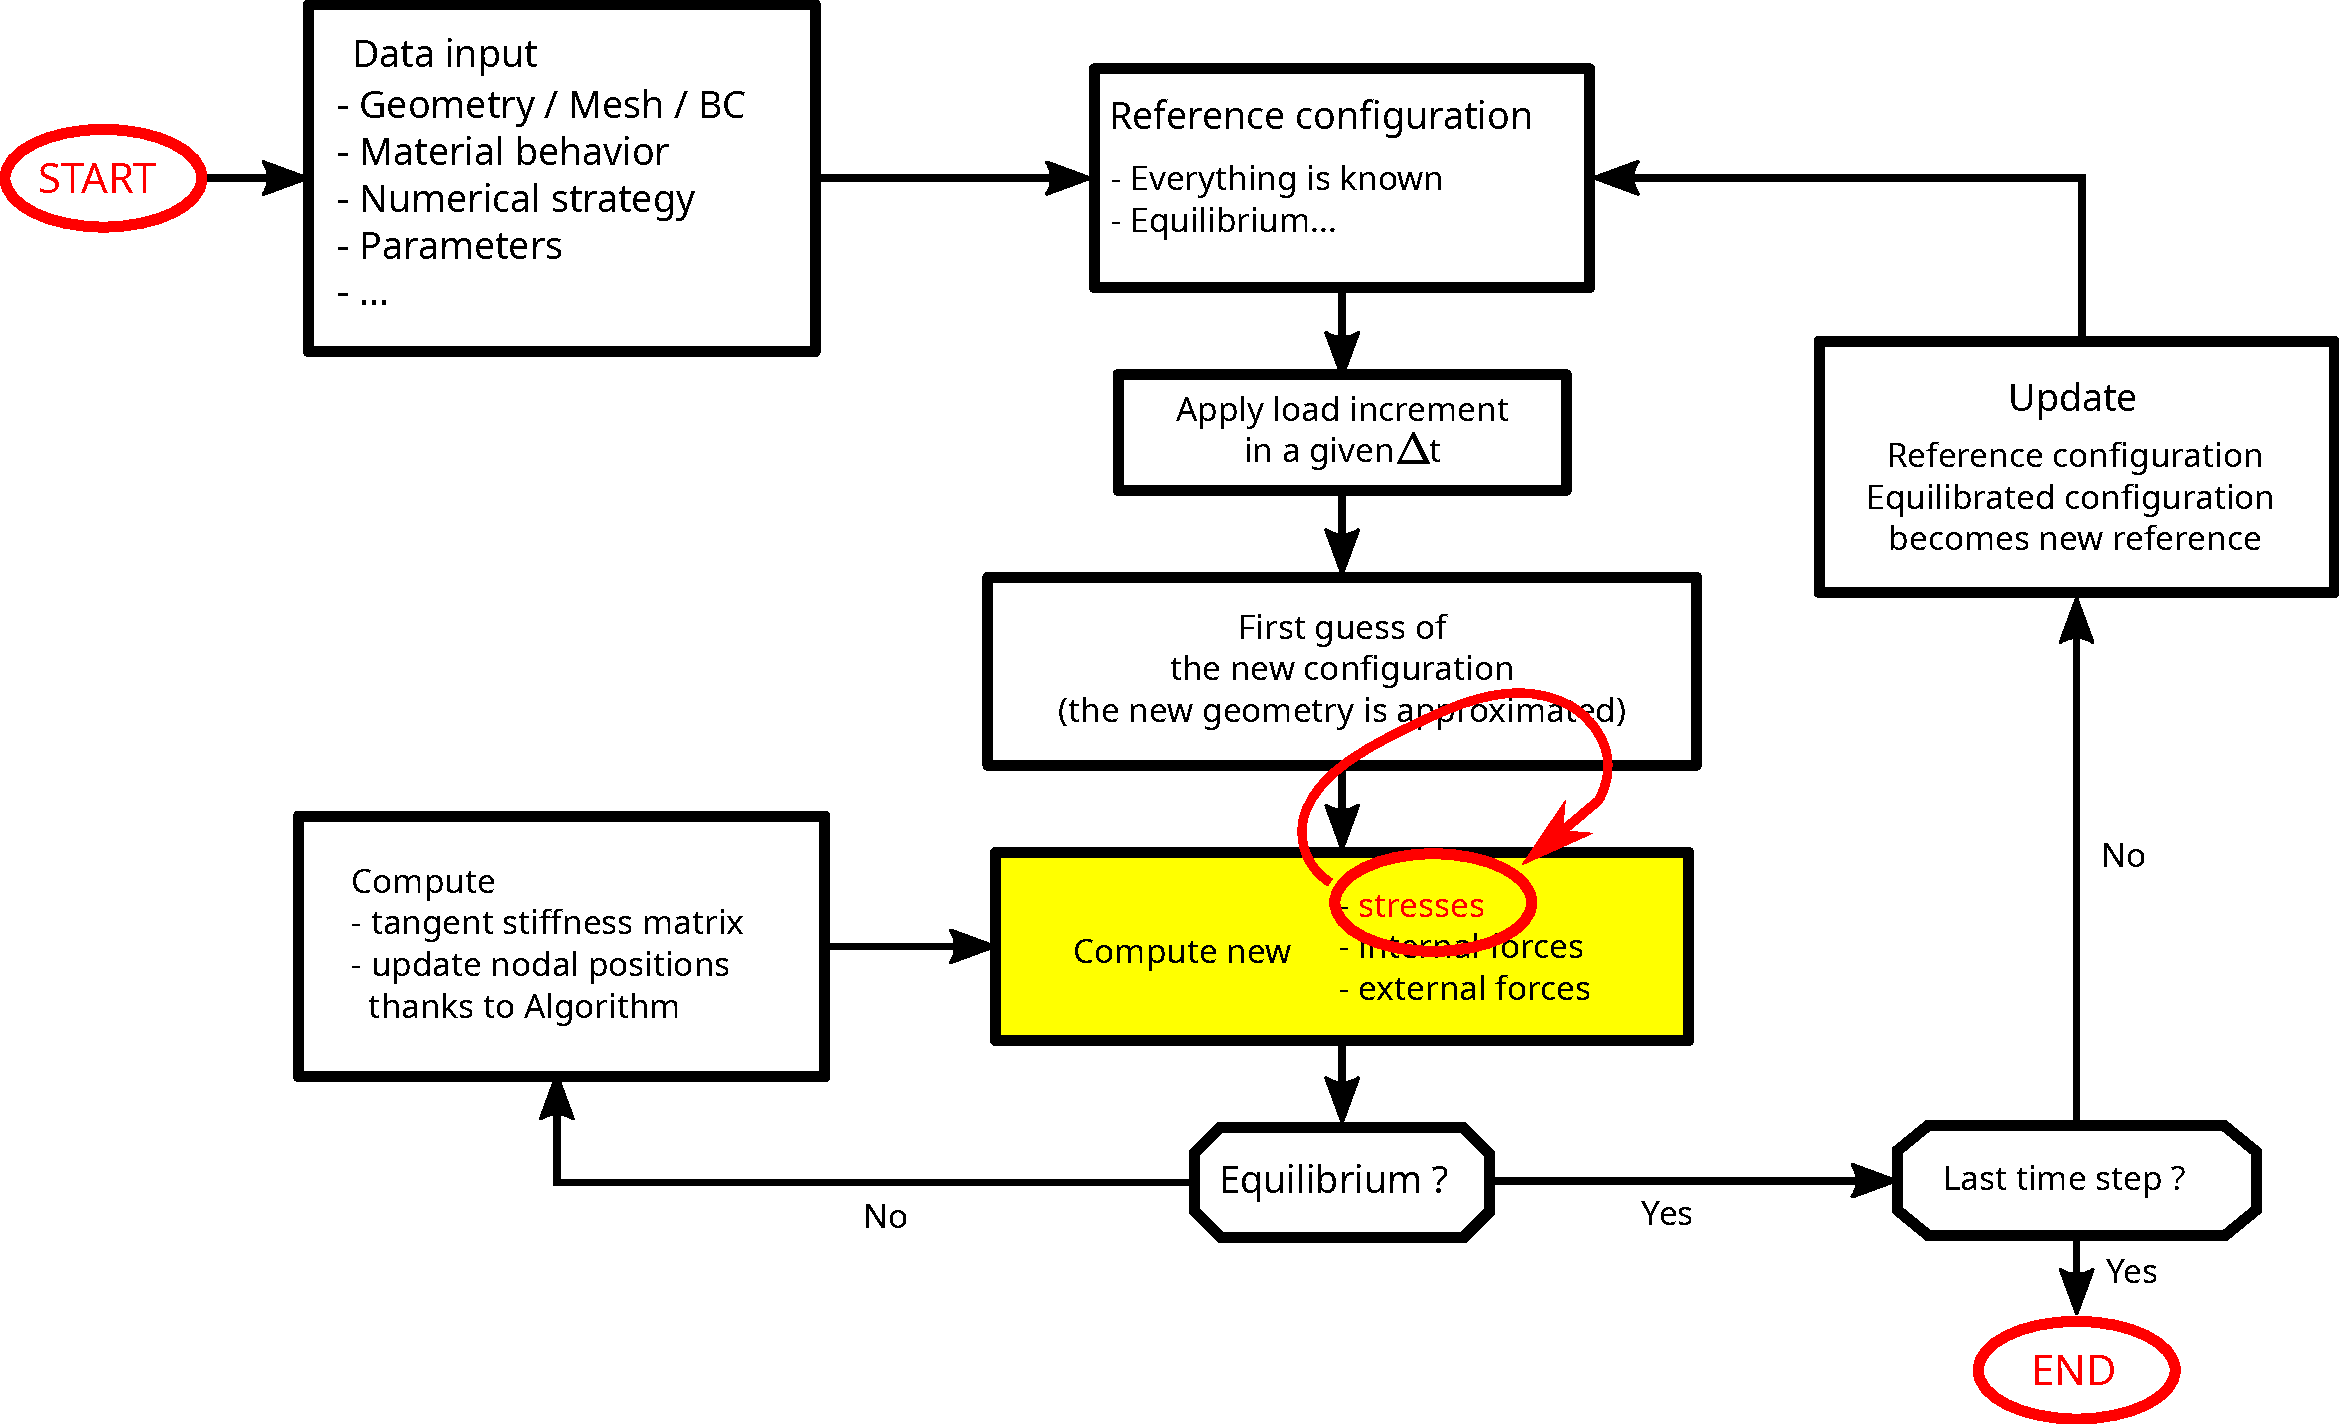
\includegraphics[width=0.9\columnwidth]{Figures/StressUpdate}
\caption{General flowchart of a FE code, focus on the stresses computation.}
\label{fig:StressUpdate}
\end{figure}

\begin{figure}[!ht]
\centering
\includegraphics[width=0.35\columnwidth]{Figures/RadialReturn}
\caption{The Radial return algorithm used to restore consistency of the stress tensor in FE simulation.}
\label{fig:RadialReturn}
\end{figure}

%------------------------------------------------------------------------------------
\section{Numerical simulations and benchmarks tests}\label{sec:Simulations}
%------------------------------------------------------------------------------------

%------------------------------------------------------------------------------------
\section{Conclusions and future work}\label{sec:Conclusions}
%------------------------------------------------------------------------------------

\reftitle{References}

% Please provide either the correct journal abbreviation (e.g. according to the “List of Title Word Abbreviations” http://www.issn.org/services/online-services/access-to-the-ltwa/) or the full name of the journal.
% Citations and References in Supplementary files are permitted provided that they also appear in the reference list here.

%=====================================
% References, variant A: external bibliography
%=====================================
\bibliography{bibliography}


% If authors have biography, please use the format below
%\section*{Short Biography of Authors}
%\bio
%{\raisebox{-0.35cm}{\includegraphics[width=3.5cm,height=5.3cm,clip,keepaspectratio]{Definitions/author1.pdf}}}
%{\textbf{Firstname Lastname} Biography of first author}
%
%\bio
%{\raisebox{-0.35cm}{\includegraphics[width=3.5cm,height=5.3cm,clip,keepaspectratio]{Definitions/author2.jpg}}}
%{\textbf{Firstname Lastname} Biography of second author}

% For the MDPI journals use author-date citation, please follow the formatting guidelines on http://www.mdpi.com/authors/references
% To cite two works by the same author: \citeauthor{ref-journal-1a} (\citeyear{ref-journal-1a}, \citeyear{ref-journal-1b}). This produces: Whittaker (1967, 1975)
% To cite two works by the same author with specific pages: \citeauthor{ref-journal-3a} (\citeyear{ref-journal-3a}, p. 328; \citeyear{ref-journal-3b}, p.475). This produces: Wong (1999, p. 328; 2000, p. 475)

%%%%%%%%%%%%%%%%%%%%%%%%%%%%%%%%%%%%%%%%%%
%% for journal Sci
%\reviewreports{\\
%Reviewer 1 comments and authors’ response\\
%Reviewer 2 comments and authors’ response\\
%Reviewer 3 comments and authors’ response
%}
%%%%%%%%%%%%%%%%%%%%%%%%%%%%%%%%%%%%%%%%%%
%\end{adjustwidth}
\end{document}

